\section{Experimental Evaluation}
In this section we experimentally evaluate  Crypt$\epsilon$  based on two parameters, the accuracy of the programs  which is measured  by reporting the expected error and the performance of Crypt$\epsilon$ programs measured via computation time. The Crypt$\epsilon$ programs considered for evaluations are the ones outlined in section \ref{program}. All the programs are compared with a competing implementation using state-of-the-art LDP techniques. 
\subsection{Accuracy}
\textit{Crypt$\epsilon$ Program 1}\\
Program 1 counts the number of records having age in range [50,60].  The competing LDP implementation uses the frequency oracle of \cite{LDP1}. 
\begin{figure}[h]
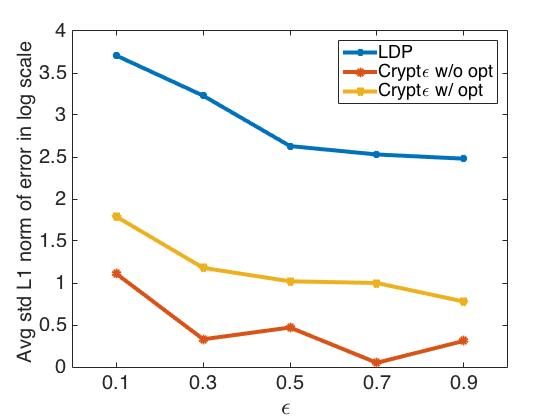
\includegraphics[width=8cm]{q1.jpg}
\caption{Comparative Accuracy Analysis for Program 1}
\end{figure}
\\\textit{Crypt$\epsilon$ Program 2}\\
\begin{figure}[h]
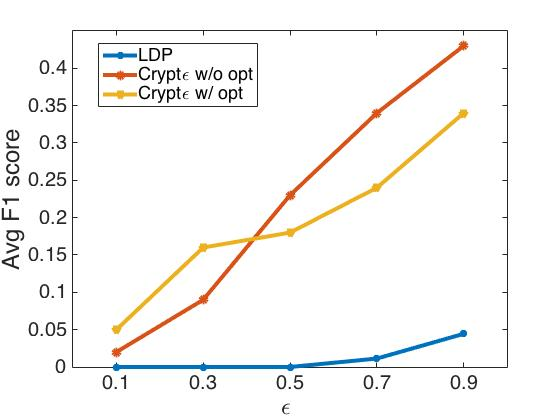
\includegraphics[width=8cm]{Q2.jpg}
\caption{Comparative Accuracy Analysis for Program 2}
\end{figure}
\textit{Crypt$\epsilon$ Program 3}\\
\textit{Crypt$\epsilon$ Program 4}\\
\textit{Crypt$\epsilon$ Program 5}\\
\textit{Crypt$\epsilon$ Program 6}\\
\textit{Crypt$\epsilon$ Program 7}\\

\subsection{Performance}
\textit{Crypt$\epsilon$ Program 1}\\
\begin{figure}[h]
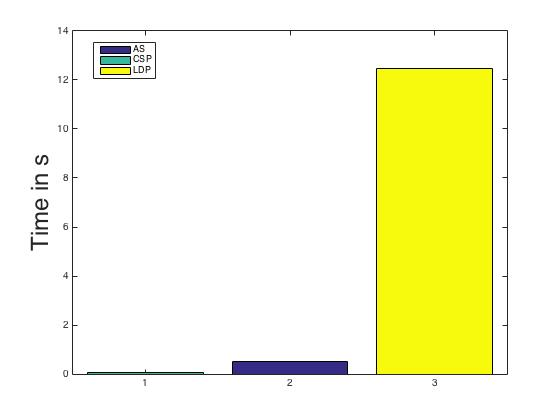
\includegraphics[width=8cm]{bar1.jpg}
\caption{Comparative Performance Analysis for Program 1}
\end{figure}
\textit{Crypt$\epsilon$ Program 2}\\\begin{figure}[h]
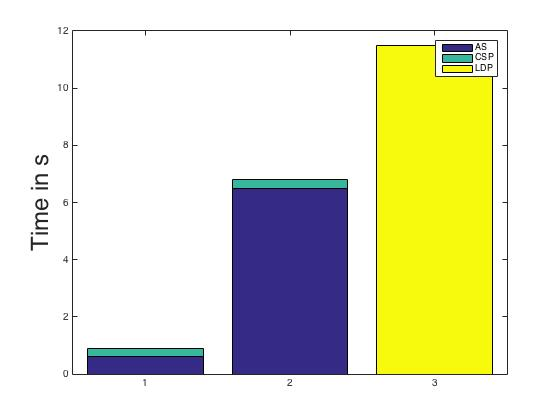
\includegraphics[width=8cm]{bar2.jpg}
\caption{Comparative Performance Analysis for Program 2}
\end{figure}
\begin{figure}[h]
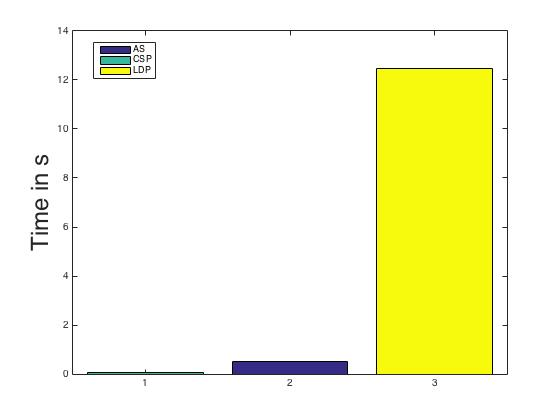
\includegraphics[width=8cm]{bar1.jpg}
\caption{Comparative Performance Analysis for Program 1}
\end{figure}
\textit{Crypt$\epsilon$ Program 3}\\
\textit{Crypt$\epsilon$ Program 4}\\
\textit{Crypt$\epsilon$ Program 5}\\
\textit{Crypt$\epsilon$ Program 6}\\
\textit{Crypt$\epsilon$ Program 7}\\



